\chapter{La polarisation}
\section{État de polarisation}
On se rappelle que la notion d'onde est dérivée des équations de Maxwell
\begin{equation}
\rot\rot\vec{\mathcal{E}} = -\mu_0\epsilon_0\dfrac{\partial^2\vec{\mathcal{E}}}{\partial t^2}\qquad\Leftrightarrow
\qquad \Delta\mathcal{E}= \mu_0\epsilon_0\dfrac{\partial^2\mathcal{E}}{\partial t^2}
\end{equation}
où l'on a considéré une équation scalaire et non vectorielle par facilité : $\mathcal{E} = \mathcal{E}_x
,\mathcal{E}_y, \mathcal{E}_z$. Cette équation possède une solution d'onde plane 
\begin{equation}
\mathcal{E} = E^{ikz}e^{-i\omega t} + c.c.
\end{equation}
où on a considéré l'axe $z$ et où l'on n'a pas utilisé pour une fois les phaseurs mais une autre approche disant 
que le champ \textbf{réel}\footnote{Car on rajoute le complexe conjugué.} $\mathcal{E}$ n'est que le champ écrit 
sous forme de phaseur additionné à son complexe conjugué, c.c. Sous forme vectorielle
\begin{equation}
\vec{\mathcal{E}} = (E_x\vec{1_x}+E_y\vec{1_y}+E_z\vec{1_z})e^{ikz}e^{-i\omega t} + c.c.
\end{equation}
où les $E_i\in\mathbb{C}$ (ceci permet d'avoir un déphasage entre les composantes du champ). On sait que
\begin{equation}
\div \vec{\mathcal{E}} = ikE_z e^{ikz}e^{-i\omega t} = 0\qquad\Rightarrow\qquad E_z=0
\end{equation}

	\begin{wrapfigure}[11]{r}{3.5cm}
	\vspace{-5mm}
	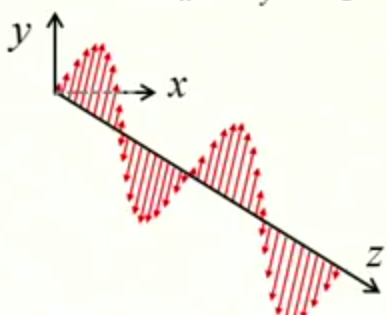
\includegraphics[scale=0.23]{ch5/image1.png}
	\captionof{figure}{ }
	\end{wrapfigure}
Une onde électromagnétique est dite \textit{transverse}
\begin{equation}
\hookrightarrow \vec{\mathcal{E}} = (E_x\vec{1_x}+E_y\vec{1_y})e^{ikz}e^{-i\omega t} + c.c.
\end{equation}
On observe bien sur le schéma ci-contre que l'amplitude possède une composante selon $x$ et $y$ : il 
s'agit d'une polarisation \textit{linéaire}.

	\subsection{Évolution du champ électrique d'une onde plane}
	Reprenons l'onde plane transverse se déplaçant le long de l'axe $z$
	\begin{equation}
	\vec{\mathcal{E}} = (E_x\vec{1_x}+E_y\vec{1_y})e^{ikz}e^{-i\omega t} + c.c.
	\end{equation}
	où $E_i\in\mathbb{C}$ : on peut les réécrire sous une forme polaire
	\begin{equation}
	E_x = \frac{1}{2}A_x e^{i\phi_x},\qquad\qquad E_y = \frac{1}{2}A_x e^{i\phi_y}
	\end{equation}
	où le facteur $1/2$ permet de faire apparaître un cosinus. 	Après substitution 
	(\danger\ ne pas oublier le c.c. sinon pas de cosinus et $\mathcal{E}\notin\mathbb{R}$ !)
	\begin{equation}
	\mathcal{E}_x = \frac{1}{2}A_x e^{i(kz-\omega t\phi_x)} + c.c.,\qquad\Leftrightarrow\qquad 
	\mathcal{E}_x = A_x\cos(kz-\omega t +\phi_x)
	\end{equation}
	On obtient similairement
	\begin{equation}
	\left\{\begin{array}{lll}
	\mathcal{E}_x &= A_x\cos(kz-\omega t +\phi_x) &= A_x\cos(\alpha)\\
	\mathcal{E}_y &= A_y\cos(kz-\omega t +\phi_y) &= A_y\cos(\alpha+\underbrace{\phi_y-\phi_x}_{\delta})\\
	\end{array}\right.
	\end{equation}
	
	\begin{wrapfigure}[9]{r}{4.5cm}
	\vspace{-9mm}
	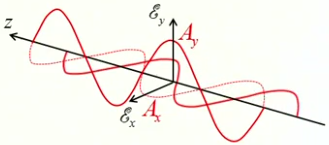
\includegraphics[scale=0.4]{ch5/image2.png}
	\captionof{figure}{ }
	\end{wrapfigure}
	Ceci représente une évolution du champ électrique, pas spécialement évidente à décrire. 
	En les traçant et en les sommant, on retrouve ci-contre pour $\phi_i=0$, l'évolution linéaire 
	(en pointillé ci-contre). 
	Si l'on considère $\phi_x\neq0,\phi_y=0$, il faut "reculer" le cosinus sur l'axe $z$ : on 
	a bien une avance de phase en $x$ (en trait plein ci-contre) et le champ ne s'annule plus nul 
	part.\\
	
	\begin{wrapfigure}[9]{l}{4cm}
	\vspace{-5mm}
	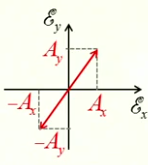
\includegraphics[scale=0.6]{ch5/image3.png}
	\captionof{figure}{ }
	\end{wrapfigure}	
	Pour se simplifier, posons que l'argument du cosinus dans l'expression de $\mathcal{E}_x$ est 
	$\alpha$ : il représente la distance parcourue sur l'axe $z$ si le temps est fixé, à une 
	constante près. Pour un $z$ donné, $\alpha$ représente le temps avec un signe moins et toujours 
	à une constante près. Prenons comme premier exemple, un déphasage nul $\delta = \phi_y-\phi_x=0$.
	Cherchons le lien entre $\mathcal{E}_x$ et $\mathcal{E}_y$ en effectuant le rapport suivant
	\begin{equation}
	\dfrac{\mathcal{E}_y}{\mathcal{E}_x} = \dfrac{A_y}{A_x}\qquad\Rightarrow\qquad \mathcal{E}_y = 
	\dfrac{A_y}{A_x}\mathcal{E}_x
	\end{equation}
	Cette linéarité est représentée ci-dessus. Les flèches représentent "l'oscillation" du champ 
	électrique. Il s'agit encore une fois de la \textit{polarisation linéaire} qui est caractérisée 
	par une certaine amplitude et un certain angle par rapport à l'axe.\\
	
	Considérons un autre exemple : $\delta=\phi_y-\phi_x=\frac{\pi}{2}$, soit un quart de période 
	de l'évolution des composantes. Cette situation ne donne aucun nœud, le champ ne s'annule plus.
	En substituant $\delta$
	\begin{equation}
	\left\{\begin{array}{ll}
	\mathcal{E}_x &= A_x\cos(\alpha)\\
	\mathcal{E}_y &= -A_y\sin(\alpha)
	\end{array}\right.
	\end{equation}
	En éliminant $\alpha$ de cette évolution paramétrique du champ, nous obtenons le lieu des points 
	qu'occupera le champ électrique :
	
 	\begin{wrapfigure}[5]{r}{3.2cm}
	\vspace{-5mm}
	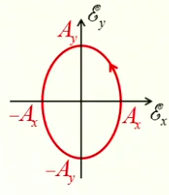
\includegraphics[scale=0.5]{ch5/image4.png}
	\captionof{figure}{ }
	\end{wrapfigure}	
	\begin{equation}
	\left(\frac{\mathcal{E}_x}{A_x}\right)^2+\left(\frac{\mathcal{E}_y}{A_y}\right)^2 = 1
	\end{equation}
	
	Il s'agit de l'équation d'une ellipse. Reste à savoir comment le champ agit dynamiquement : 
	dans quel sens "tourne-t-on" sur cette ellipse. Rappelons-nous : $\alpha = kz-\omega+\phi_x$. On 
	s'intéresse à la composante temporelle : si $z=\phi_x=0$, $\alpha \propto -t$. Quand le temps 
	évolue, on observe une diminution progressive de la composante en $x$ à partir de 1 et le comportement 
	inverse pour le composante en $y$, ayant un sinus. Le point de départ est 1 pour le cosinus et 0 
	pour le sinus, la rotation se fera dans le sens trigonométrique positif. Si l'on applique la 
	règle de la main droite pour déterminer la direction de l'axe $z$, les doigts vont dans le même 
	sens que la rotation sur l'ellipse : il s'agit d'une \textit{polarisation elliptique droite}.\\
	
 	\begin{wrapfigure}[7]{r}{5.5cm}
	\vspace{-5mm}
	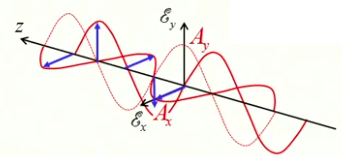
\includegraphics[scale=0.5]{ch5/image5.png}
	\captionof{figure}{ }
	\end{wrapfigure}	
	Regardons ceci géométriquement, en représentant les vecteurs résultants en bleu. On remarque 
	que si on effectue la règle de la main droite, en $z$, il tourne dans l'autre sens (le pouce 
	est opposé à l'axe $z$). C'est normal, l'évolution temporelle d'une onde progressive est inversée 
	par rapport à se composante spatiale. Un polarisation est dite \textit{droite} lorsqu'elle tourne 
	dans le sens horlogique lorsqu'on s'éloigne en $z$ : le sens de rotation en $z$ sera opposé à 
	sa rotation en $t$.\\
	
	Si $A_x=A_y$, on obtient une \textit{polarisation circulaire droite}. Si on considère $\delta = 
	-\frac{\pi}{2}$ on se trouve dans le cas d'un retard de phase. Le champ est spatialement 
	dextrogyre : il faut inverser le sens de la polarisation est alors dit \textit{gauche} (avec la
	règle de la main gauche, on obtiendrait l'axe $z$, petit moyen mnémotechnique).\\
	
	Cessons-en maintenant avec les exemples et considérons le cas général. Pour se faire, effectuons
	$\cos(a+b)$ dans l'expression $\mathcal{E}_y$
	\begin{equation}
	\frac{\mathcal{E}_x}{A_y} = \underbrace{\cos\alpha}_{\mathcal{E}_x/A_x}\cos\delta-\sin\alpha\sin\delta
	\end{equation}
	où l'on utilise la première expression (celle de $\mathcal{E}_x$) et le fait que $\DS \sin\alpha = 
	\sqrt{1-\left(\frac{\mathcal{E}_x}{A_x}\right)}$. On trouve alors
	\begin{equation}
	\frac{\mathcal{E}_y}{A_y} = \frac{\mathcal{E}_x}{A_x}\cos\delta -\sqrt{1-\left(\frac{\mathcal{E}_x}{
	A_x}\right)^2}\sin\delta
	\end{equation}
	N'ayant plus de $\alpha$, il s'agit bien du lieu des points de l'extrémité du vecteur du champ électrique. 
	Analysons ceci en commençant par passer la racine à gauche et en élevant tout au carré
	\begin{equation}
	\sqrt{1-\left(\frac{\mathcal{E}_x}{A_x}\right)^2}\sin\delta = \frac{\mathcal{E}_x}{A_x}\cos\delta -
	\frac{\mathcal{E}_y}{A_y} 
	\end{equation}
	Dès lors, en effectuant le produit remarquable
	\begin{equation}
	\left[1-\left(\frac{\mathcal{E}_x}{A_x}\right)\right]\sin^2\delta = \left(\frac{\mathcal{E}_x}{A_x}\right)^2
	\cos^2\delta +\left(\frac{\mathcal{E}_y}{A_y}\right)^2- 2\frac{\mathcal{E}_x\mathcal{E}_y}{A_xA_y}\cos\delta
	\end{equation}
	En simplifiant l'identité fondamentale trigonométrique
	\begin{equation}
	\sin^2\delta = \left(\frac{\mathcal{E}_x}{A_x}\right)^2
	+\left(\frac{\mathcal{E}_y}{A_y}\right)^2- 2\frac{\mathcal{E}_x\mathcal{E}_y}{A_xA_y}\cos\delta
	\end{equation}
	
		\begin{wrapfigure}[2]{r}{4.5cm}
	\vspace{-12mm}
	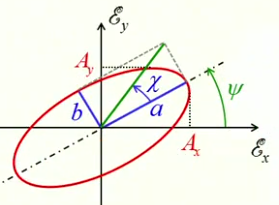
\includegraphics[scale=0.5]{ch5/image6.png}
	\captionof{figure}{ }
	\end{wrapfigure}
	Il s'agit de l'équation d'une conique qui n'est rien d'autre qu'une ellipse. Il s'agit du cas de 
	polarisation le plus général portant le doux nom d'\textit{ellipse de polarisation}. Celle-ci aura 
	une certaine inclinaison $\psi$ repérée par rapport à l'axe $x$. Sans rentrer dans les détails, on 
	peut montrer que
	\begin{equation}
	\psi = \frac{1}{2}\arctan\left[\dfrac{2A_xA_y}{A_x^2-A_y^2}\cos\delta\right]
	\end{equation}
	La différence avec les secondaires et qu'à la place d'utiliser $a$ et $b$ pour le grand/petit axe, 
	on utilise l'ellipticité $\chi$ donné par (non démontré ici)
	\begin{equation}
	\chi = \frac{1}{2}\arcsin\left[\dfrac{2A_xA_y}{A_x^2+A_y^2}\sin\delta\right]
	\end{equation}
	L’ellipse de polarisation, et donc l'état de polarisation, sera décrite par son inclinaison et 
	son ellipticité. Par construction $\chi=\arctan(b/a)$ où $|b|<a$ (si $b>0$ la polarisation sera 
	droite) et donc $|\chi| \leq  \frac{\pi}{4} \rightarrow \chi <0$ représente une polarisation 
	elliptique gauche.\\
	
	Prenons un exemple : $\delta = 0\rightarrow \chi = 0\rightarrow b = 0$ et l'ellipse se réduit à 
	une droite. Une ellipticité nulle indique que l'on se trouve dans le cadre d'une polarisation 
	linéaire. Pour l'inclinaison 
	\begin{equation}
	\tan(2\psi) = \left[\frac{2A_y/A_x}{1-A_y^2/A_x^2}\right] = \dfrac{2\tan\psi}{1-\tan^2\psi}
	\end{equation}
	où l'on a utilisé la formule de l'angle double. Par identification $A_y/A_x = \tan\psi$ ce qui 
	est bien le résultat précédemment obtenu.\\
	
	\begin{wrapfigure}[6]{l}{4cm}
	\vspace{-9mm}
	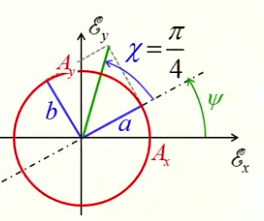
\includegraphics[scale=0.34]{ch5/image7.png}
	\captionof{figure}{ }
	\end{wrapfigure}
	Soif de savoir, partons sur un nouvel exemple : $\delta = \frac{\pi}{2}, A_y=A_x \rightarrow 
	\chi = \frac{\pi}{4}\rightarrow a=b=A_x$. Il s'agit de la polarisation circulaire droite, 
	$\chi$ étant positif. Pour le calcul de l'inclinaison, on obtient une indétermination ($\psi = 0/0$)
	ce qui est cohérent : l'inclinaison d'un cercle est indéterminée. La fin de la vidéo propose quelques 
	petites illustrations animées.
	
	
	
	
	
	
	
	
	
	
	
	
	
	
	
	
	
	
	
	
	
	
	
	
	
	
	
	
	